\documentclass[margin=5mm, tikz]{standalone}
\usepackage[utf8x]{inputenc}
\usepackage{tikz}
\begin{document}
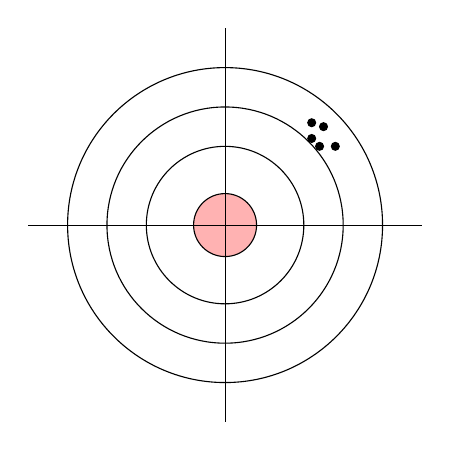
\begin{tikzpicture}
    
    \draw [fill=red!30] (0, 0) circle (0.4);
    \foreach \y in {1, 1.5, 2}
        \draw (0, 0) circle (\y);
    
    
    % Medida precisa pero no exacta
    \draw [fill] (1.25, 1.25) circle (0.05);
    \draw [fill] (1.1, 1.1) circle (0.05);
    \draw [fill] (1.1, 1.3) circle (0.05);
    \draw [fill] (1.2, 1) circle (0.05);
    \draw [fill] (1.4, 1) circle (0.05);



    \draw (-2.5, 0) -- (2.5, 0);
    \draw (0, -2.5) -- (0, 2.5);
\end{tikzpicture}
\end{document}